\documentclass{article}

\usepackage{tikz} 
\usetikzlibrary{automata, positioning, arrows} 
\usepackage{amsthm}
\usepackage{amsfonts}
\usepackage{amsmath}
\usepackage{amssymb}
\usepackage{fullpage}
\usepackage{color}
\usepackage{parskip}
\usepackage{hyperref}
\usepackage{bookmark}
  \hypersetup{
    colorlinks = true,
    urlcolor = blue,       % color of external links using \href
    linkcolor= blue,       % color of internal links 
    citecolor= blue,       % color of links to bibliography
    filecolor= blue,        % color of file links
    }
    
\usepackage{listings}
\usepackage{graphicx}
\definecolor{dkgreen}{rgb}{0,0.6,0}
\definecolor{gray}{rgb}{0.5,0.5,0.5}
\definecolor{mauve}{rgb}{0.58,0,0.82}
\usepackage{etoolbox}
\AtBeginEnvironment{align}{\setcounter{equation}{0}}


\lstset{frame=tb,
  language=haskell,
  aboveskip=3mm,
  belowskip=3mm,
  showstringspaces=false,
  columns=flexible,
  basicstyle={\small\ttfamily},
  numbers=none,
  numberstyle=\tiny\color{gray},
  keywordstyle=\color{blue},
  commentstyle=\color{dkgreen},
  stringstyle=\color{mauve},
  breaklines=true,
  breakatwhitespace=true,
  tabsize=3
}

\newtheoremstyle{theorem}
  {\topsep}   % ABOVESPACE
  {\topsep}   % BELOWSPACE
  {\itshape\/}  % BODYFONT
  {0pt}       % INDENT (empty value is the same as 0pt)
  {\bfseries} % HEADFONT
  {.}         % HEADPUNCT
  {5pt plus 1pt minus 1pt} % HEADSPACE
  {}          % CUSTOM-HEAD-SPEC
\theoremstyle{theorem} 
   \newtheorem{theorem}{Theorem}[section]
   \newtheorem{corollary}[theorem]{Corollary}
   \newtheorem{lemma}[theorem]{Lemma}
   \newtheorem{proposition}[theorem]{Proposition}
\theoremstyle{definition}
   \newtheorem{definition}[theorem]{Definition}
   \newtheorem{example}[theorem]{Example}
\theoremstyle{remark}    
  \newtheorem{remark}[theorem]{Remark}

\title{CPSC-354 Report}
\author{Brandon Hughes \\ Chapman University}

\date{\today} 

\begin{document}

\maketitle

\begin{abstract}
  This report reflects on how theoretical concepts like parsing, recursion, and Turing completeness 
  were integrated into practical programming tasks. Through assignments and group projects, we explored 
  how these ideas connect to software engineering, such as building interpreters and solving logic puzzles.
  Along the way, we faced challenges like managing grammar precedence, understanding capture-avoiding 
  substitution, and applying lambda calculus, which pushed us to think critically and adapt. Working 
  together as a team was key to overcoming these difficulties and deepened our understanding of 
  programming language mechanics. Overall, this course gave us valuable insights into the theoretical 
  foundations of programming languages and showed how they apply to real-world scenarios.
\end{abstract}

\setcounter{tocdepth}{3}
\tableofcontents

\section{Introduction}\label{intro}

This report reflects on the concepts and experiences gained while taking programming languages at 
Chapman University. The course aims to understand the creation of programming languages, how they work, 
and to be able to design a basic programming language through accepting expressions. By combining a 
practical and a theoretical component into our coursework, we were able to gain a perspective on how the 
foundations of programming languages depend on topics like recursion, parking, and lambda calculus to 
connect to a larger field of software engineering.

The report is organized by having weekly updates added onto the report, a summary of important lessons 
from our two group assignments and project, and lastly a conclusion of topics learned, what we liked, 
and improvements to be made. Each weekly update contains a summary of the notes given in class and 
through other learning such as videos and books, a homework assignment assigned and completed, and 
a higher-level question regarding the information provided to be answered or proposed. The lessons 
contain a detailed reflection on key concepts and how they are applied to the program we created, as 
well as challenges faced during the creation of the programs and how we were able to overcome them by 
working together.

Understanding the theoretical portions assisted with the writing of interpreters and gained an outlook 
on some of the questions guiding programming language research. The practical portion was applying those 
theories to building multiple projects that will be extended to a larger functional and/or imperative 
programming language.

Personally, while the course was ultimately challenging to understand multiple theorems and apply 
them to our own projects through repetition or creating new ideas, it pushed me to think critically 
about problems and approach programming from a different perspective.

\section{Week by Week}\label{homework}

\subsection{Week 1}

\subsubsection{Notes}

During this week, there was a review of Git and being introduced to Latex and Lean. Some helpful commands include git add, commit, status, and push. 
Through the website "https://sudorealm.com/blog/how-to-write-latex-documents-with-visual-studio-code-on-mac", we set up latex to be able to complete the weekly report.

\subsubsection{Homework} 

1. Finish the Natural Number Game Tutorial World. \\
\hspace*{2em}a) Show the completed work for levels 5 through 8. \\
\hspace*{2em}b) For one level, explain in detail how the Lean proof is related to its corresponding proof in mathematics. \\

1a. Show the completed work for levels 5 through 8. \\
Level 5: Prove that a+(b+0)+(c+0)=a+b+c.
\begin{lstlisting}
rw[add_zero]
rw[add_zero]
rfl
\end{lstlisting}

Level 6: Prove that a+(b+0)+(c+0)=a+b+c.
\begin{lstlisting}
repeat rw[add_zero]
rfl
\end{lstlisting}

Level 7: Prove that for all natural numbers a, we have succ(a)=a+1.
\begin{lstlisting}
rw[one_eq_succ_zero]
rw[add_succ]
rw[add_zero]
rfl
\end{lstlisting}

Level 8: Prove that 2+2=4.
\begin{lstlisting}
repeat rw[four_eq_succ_three, three_eq_succ_two, two_eq_succ_one, one_eq_succ_zero]
repeat rw[add_succ, add_succ, add_zero]
rfl
\end{lstlisting}

1b. For one level, explain in detail how the Lean proof is related to its corresponding proof in mathematics. \\
For level 7, we had to prove the therom of the succ(n) is also equal to n+1. 

Lean Proof:
\begin{lstlisting}
Start: succ(n) = n + 1
  1: rw[one_eq_succ_zero]
  Result: succ n = n + succ 0
  2: rw[add_succ]
  Result: succ n = succ (n + 0)
  3: rw[add_zero]
End: succ n = succ n

Thus, proving reflexitivity. 
\end{lstlisting}

Proof by Mathematics: By using the induction we are able to prove the therom of the succ(a) is equal to a+1.
\begin{lstlisting}
Base Case:
  Consider n = 0,

  S(0) = 0 + 1

  0 + 1 = 1

  Thus, 0 + 1 = S(0), which holds true.

Inductive hypothesis:

  Assume for some natural number k that k + 1 = S(k).

Inductive Step:

  We need to show that k + 1 + 1 = S(k + 1).

  (k + 1) + 1 = S(k + 1), by adding parenthesis

  S(k) + 1 = S(k + 1), by using the inductive hypothesis.

  S(k + 1) = S(k + 1), by using addition of successors.

Thus, proving reflexitivity.
\end{lstlisting}

Through these steps, we can see that the end goal of proving reflexitivity on both the Lean proof and its corresponding proof in mathematics. The similarites come from the lean proof and the inductive step however,
as they are similar steps in being able to prove the theorem. The lean proof is more straight forward because instead of proving it through a basis, inductive hypothesis, and inductive step, you only have to prove
it through rewriting the equation so that both sides are equal. Which is done through the indutive step of the mathematics proof. 

\subsubsection{Comments and Questions}

When looking at Formal Systems from the textbook, we are given this example of an impossible puzzle to solve. 
The MU problem, where you are given a set of rules and have to obtain MU from MI, however, its impossible because you can never end up without 
having an odd number of I's inside the string. When it comes to Formal systems, and solving them a lot of times people will look towards actually doing 
compared to trying to assess the logic behind this however computers, mostly AI, generally start at the logic. How might combining human intuition and AI's 
logical reasoning lead to more effective problem-solving strategies? Would we be able to solve problems quicker, our would AI's logical reasoning overtake the 
human trial and error method?

\subsection{Week 2}

\subsubsection{Notes}

During this week, we learned in class that both Math and Lean can be seen as langauges. Math is a specification language while Lean is a programming language. A
specification langauge is used to define the requirements and properties of a system. A Math proof can be written into Lean proof very easily since they use and
follow the same rules when it comes to solving thoerems and problems. The difference between the two proofs however is that in Math we typically reason forwards
from the problem to the answer, while in Lean we reason backwards from the answer to the problem. We could also do it the opposite way but it would become more
challengening. Another idea that we learned in class is that a recursive data type, which could also be called an algebraic data type, and induction are of 
similar processes as you define what a number is inside of a number. An example of recursion can be seen in the Tower of Hanoi as you are solving the previous
tree in the next tree. Tower of Hanoi are also similar to binary search trees since the amount of nodes in a amount of 'n' level of a tree, if you have a balanced
tree is the same amount of moves it takes to solve when you have ;n' amount of disks. Lastly, we also learned that when you write a recursive program it creates 
a stack behind the scenes to solve all the problems, it will always go to the one on top rather than starting back at the start of the problem. If you don't have
a stack you could also write it on a rewriting machine.

\subsubsection{Homework}

1. Finish the Natural Number Game Addition World. \\
\hspace*{2em}a) Show the completed work for levels 1 through 5. \\
\hspace*{2em}b) For level 4 or 5, explain in some detail how the Lean proof is related to its corresponding proof in mathematics \\

1a.\\
Level 1:
\begin{align*}
  Sd&=Sd & \texttt{rfl} \\
  S(0+d)&=Sd & \texttt{rw[hd]} \\
  0+Sd &= Sd & \texttt{rw[add\_succ]} \\
  0&=0 & \texttt{rfl} \\
  0+0 &= 0 & \texttt{rw[add\_zero]} \\
  0+n &= n & \texttt{induction n with d hd} \\
\end{align*}

Level 2:
\begin{align*}
  SS(a+d)&=SS(a+d) & \texttt{rfl} \\
  S(Sa+d)&=SS(a+d) & \texttt{hd} \\
  S(Sa+d)&=S(a+Sd) & \texttt{rw[add\_succ]} \\
  Sa+Sd&=S(a+Sd) & \texttt{rw[add\_succ]} \\
  Sa&=Sa & \texttt{rfl} \\
  Sa&=S(a+0) & \texttt{rw[add\_zero]} \\
  Sa+0&=S(a+0) & \texttt{rw[add\_zero]} \\
  Sa+b&=S(a+b) & \texttt{induction b with d hd} \\
\end{align*}

Level 3:
\begin{align*}
  S(d+a)&=S(d+a) & \texttt{rfl} \\
  S(a+d)&=S(d+a) & \texttt{rw[hd]} \\
  S(a+d)&=Sd+a & \texttt{rw[succ\_add]} \\
  a+Sd&=Sd+a & \texttt{rw[add\_succ]} \\
  a&=a & \texttt{rfl} \\
  a&=0+a & \texttt{rw[zero\_add]} \\
  a+0&=0+a & \texttt{rw[add\_zero]} \\
  a+b&=b+a & \texttt{induction b with d hd} \\
\end{align*}

Level 4:
\begin{align*}
  S(a+(b+d))&=S(a+(b+d)) & \texttt{rfl} \\
  S(a+b+d)&=S(a+(b+d)) & \texttt{rw[hd]} \\
  S(a+b+d)&=a+S(b+d) & \texttt{rw[add\_succ]} \\
  S(a+b+d)&=a+(b+Sd) & \texttt{rw[add\_succ]} \\
  a+b+Sd&=a+(b+Sd) & \texttt{rw[add\_succ]} \\
  a+b&=a+b & \texttt{rfl} \\
  a+b&=a+(b+0) & \texttt{rw[add\_zero]} \\
  a+b+0&=a+(b+0) & \texttt{rw[add\_zero]} \\
  a+b+c&=a+(b+c) & \texttt{induction c with d hd} \\
\end{align*}

Level 5:
\begin{align*}
  S(a+d+b)&=S(a+d+b) & \texttt{rfl} \\
  S(a+b+d)&=S(a+d+b)  & \texttt{rw[hd]} \\
  S(a+d+b)&=S(a+d)+b & \texttt{rw[succ\_add]} \\
  S(a+d+b)&=a+Sd+b & \texttt{rw[add\_succ]} \\
  a+b+Sd&=a+Sd+b & \texttt{rw[add\_succ]} \\
  a+b&=a+b & \texttt{rfl} \\
  a+b&=a+0+b & \texttt{rw[add\_zero]} \\
  a+b+0&=a+0+b & \texttt{rw[add\_zero]} \\
  a+b+c&=a+c+b & \texttt{induction c with d hd} \\
\end{align*}

1b. \\

For Level 4, we are proving the associativity of addition. 
On the set of natural numbers, addition is associative. 
In other words, if a,b and c are arbitrary natural numbers, we have (a+b)+c=a+(b+c).
In Math and Lean, we have to do a proof by induction on c.\\ 

Math Proof:\\ 
\begin{align*}
  (a+b)+c&=a+(b+c) \\
\end{align*}
Base Case: $(a+b)+0=a+(b+0)$\\ 
\begin{align*}
  (a+b)+0&=a+(b+0)\\
  a+b&=a+(b+0) & \text{ def of } +\\
  a+b&=a+b & \text{ def of } +\\
\end{align*}

Induction Step: $(a+b)+Sd=a+(b+Sd)$ \\

Induction Hypothesis: $(a+b)+d=a+(b+d)$ \\

\begin{align*}
  (a+b)+Sd&=a+(b+Sd)\\
  S((a+b)+d)&=a+(b+Sd) & \text{ def of } +\\
  S((a+b)+d)&=a+S(b+d) & \text{ def of } +\\
  S((a+b)+d)&=S(a+(b+d)) & \text{ def of } +\\
  S(a+(b+d))&=S(a+(b+d)) & \text{ Induction Hypothesis}\\
\end{align*}

The Lean proof written above is the exact same as the same steps in the Math proof just backwards. 
Instead of having add\_zero and add\_succ, we have the definition of addition as that can be proven to add both 
successors and zero to numbers.  

\subsubsection{Comments and Questions}

In the beginning of the reading, it takes about how recursion is different from paradox or infinite regress, since it  never defines somethin in terms of iteself, but always in terms of simpler versions of itself. Is the only difference between a paradox and a recursively solveable problem be that it has an exit statement at its very simplest version or are there more differences? If some paradoxs were proposed recursively, would we be able to break down some harder problems into simpler version to prove if they are unsolveable logically?

\subsection{Week 3}

\subsubsection{Homework}

For this homework assignment, I used ChatGPT to explore language interoperability, which refers to how different programming languages interact with one another to create a single system or application. In modern software development and application creation, it is common for multiple programming languages to be used together to meet different kinds of functions and performance requirements. As a result, being able to integrate between these languages flawless is essential for building efficient  and reliable systems. This report goes over some of the current methods used to ensure compatibility between programming languages and investigates ways to enhance these systems further. While many languages already possess some interoperability with one another, challenges arise when trying to bridge the gaps between the languages that were not designed to work together. These challenges can lead to issues such as performance inefficiencies, data type mismatches, and increase complexity in code maintenance. By examining these difficulties, potential improvements can be seen to create more solutions for the future. Additionally, advancements in tools, frameworks, and compiler technology could further enhance interoperability efforts. By improving in ways in which programming languages collaborate, developers will be able to build more versatile, efficient, and scalable systems. Addressing these challenges and making enhancements will lead to more seamless development processes and better applications.  

\href{https://github.com/Brandon-Hughes/LLM_Literature_Review}{LLM Literature Review}

\subsection{Week 4}

\subsubsection{Notes}

Concrete syntax considers a program as a string in the form of a sequence of characters. This is the syntax that we are used to seeing and interacting with on a day to day basis. 
Abstract syntax considers a program as a tree-like structure that represents the program's structure and organization. 
An Abstract Syntax Tree (AST) is a tree representation of the abstract syntactic structure of source code written in a programming language. 
ASTs can write type checkers, interpreters, and compilers via recursion on these algebraic data types, but translating strings into trees is very difficult.
The main idea is that you can translate a concrete syntax (string) into a concrete syntax tree, but translating a concrete syntax tree (string) into an abstract syntax tree (tree) is very difficult.
Parsing is about putting the parentheses in the correct position.
A context-free grammar is a set of rules that describe how to form strings in a language.
The purpose of a context-free grammar is to define a set of strings or a language, in which a particular string in the lanaguage can be derived from the start symbol. The symbols that will appear in the strings (terminals), are those that are enclosed in single quotes.
Other symbols may never appear in the parsed string, but only control which strings can be derived. These are called non-terminals.


\subsubsection{Homework}
Using the context-free grammar: 
\begin{align*}
Exp &\rightarrow Exp + Exp1 \\
Exp1 &\rightarrow Exp1 \* Exp2 \\
Exp2 &\rightarrow Integer \\
Exp2 &\rightarrow ( Exp )  \\
Exp &\rightarrow Exp1 \\
Exp1 &\rightarrow Exp2 \\    
\end{align*}

Generate the abstract syntax tree for the expressions. \\
1. 2+1 \\
2. 1+2\*3 \\
3. 1+\(2\*3\) \\
4. \(1+2\)\*3 \\
5. 1+2\*3+4\*5+6 \\

\noindent
The Abstract Syntax Trees for Problems 1 through 5 are shown below:

\includegraphics[width=0.8\textwidth]{img/HW4.jpg}

As we can see from the image above, each of the problems can be solved by using the rules of the context-free grammar with the start symbol Exp.

\subsubsection{Comments and Questions}

During this week we've explored the idea of applying context-free grammar in the basics of Math and we are going to start applying that into programming languages. Besides the usage in math and programming lanaguages, are we able to see or use context-free grammar in other examples or in our lives?

\subsection{Week 5}

\subsubsection{Notes}

By practicing the application of context-free grammars (CFG) in a programming language, a calculator was created that took an input and broke it down into an Abstract Syntax Tree (AST) using a CFG. By breaking the expression into a AST, the problem was solved by reading through the AST to produce a correct result for the expression. This application served to practice parsing expressions into smaller pieces that are more easily read by programming languages, as well as provide an introduction to context-free grammars.

The second portion of this class week focused on an introduction and tutorial of constructive logic. Through the Lean logic game, students were introduced to how to write math expressions as logic-driven trees, similar to how a CFG might break an expression into components. While the process is similar, it differs by working with logical inferences instead of numbers. The keyword "exact" is used to give the game's answer, which serves as the concluding statement. The symbol $\wedge$ denotes a logical "and," meaning the logic must follow both A and B. The logical "and" can be broken apart using the keywords ".left" and ".right" to access either the left or right item of the $\wedge$, respectively.

\subsubsection{Homework}

1. Finish the Lean Logic Game Tutorial World. \\
\hspace*{2em}a) Show the completed work for levels 1 through 8. \\
\hspace*{2em}b) For level 8, write down the proof in mathematical logic.\\

1a.\\
Level 1: If todo\_list is P, then P.
\begin{align*}
  \text{exact todo\_list}
\end{align*}

Level 2: If p is P and s is S, then P $\wedge$ S.
\begin{align*}
  \text{exact $\langle$p,s$\rangle$}
\end{align*}

Level 3: If a is A, i is I, o is O, and u is U, then A $\wedge$ I $\wedge$ O $\wedge$ U.
\begin{align*}
  \text{exact $\langle$a,$\langle$i,$\langle$o,u$\rangle$$\rangle$$\rangle$}
\end{align*}

Level 4: If vm is P $\wedge$ S, then P.
\begin{align*}
  \text{exact vm.left}
\end{align*}

Level 5: If h is P $\wedge$ Q, then Q.
\begin{align*}
  \text{exact vm.right}
\end{align*}

Level 6: If h1 is A $\wedge$ I and h2 is O $\wedge$ U, then A $\wedge$ U.
\begin{align*}
  \text{exact $\langle$h1.left,h2.right$\rangle$}
\end{align*}

Level 7: If h is (L $\wedge$ ((L $\wedge$ C) $\wedge$ L) $\wedge$ L $\wedge$ L $\wedge$ L), then C.
\begin{align*}
  \text{exact h.left.right.left.left.right}
\end{align*}

1b. 

Level 8: If ((P $\wedge$ S) $\wedge$ A) $\wedge$ $\neg$I $\wedge$ (C $\wedge$ $\neg$O) $\wedge$ $\neg$U then A $\wedge$ C $\wedge$ P $\wedge$ S

\begin{align}
  \text{assumption1} &: ((P \wedge S) \wedge A) \wedge \neg I \wedge (C \wedge \neg O) \wedge \neg U & \text{} \\
  A && \text{and\_left and\_right on (1)} \\
  C && \text{and\_right and\_right and\_left and\_left on (1)} \\
  P && \text{and\_left and\_left and\_left on (1)} \\
  S && \text{and\_left and\_left and\_right on (1)} \\
  A \wedge C \wedge P \wedge S && \text{and\_intro on (2) (3) (4) (5)}
\end{align}

\subsubsection{Comments and Questions}

In the creation of a context-free grammar, we can see that by establishing a hierarchy through constructs like exp, exp1, exp2, etc., we can control the order of operations. How can programmers determine how deep the hierarchy should go to ensure the grammar is well-structured and the language doesn't break?

\subsection{Week 6}

\subsubsection{Notes}

Lambda calculus is a programming language comprised of only variables and functions. Two main portions build lambda calculus, the syntax and the semantics. The syntax is made of three constructions abstraction, application, and variables. Abstraction is taking the program and using a placeholder variable so that it can change what you use. It's the creation of general-purpose functions that can take in many different inputs but will produce a structured output. Application is how we apply functions to one another. Lastly, variables are just variables. An important part of Lambda calculus is dropping the parenthesis for easier readability. You apply the left and move to the right to solve for lambda in the same parenthesis. The next portion of Lambda calculus is the semantics or how to execute it. By executing, we are either inputting numbers into variables or simplifying them into their lowest form. When having multiple inputs and variables within the same expression, apply it in the same parentheses or the farthest lambda to the left if you only have the function in one parenthesis but multiple inputs and variables. When solving problems, you may arrive at to capture avoiding substitution, when multiple inputs are being placed into a variable, many solutions act differently here it will place it into all of them while some of them place it only into the first variable possible. To solve this, they created bound and free variables where bound variables are set within the function at the beginning, while free variables are those that are inputted. 

\subsubsection{Homework}

Finish the Lean Logic Game Tutorial World. Show the completed work for levels 1 through 9. \\

Level 1: If bakery\_service is P $\rightarrow$ C, then C.
\begin{align*}
  \text{exact bakery\_service \, p}
\end{align*}

Level 2: Show that C $\rightarrow$ C.
\begin{align*}
  \text{exact } \lambda h \Rightarrow h
\end{align*}

Level 3: Show that I $\wedge$ S $\rightarrow$ S $\wedge$ I.
\begin{align*}
  \text{exact } \lambda h \Rightarrow \langle h.right , h.left\rangle
\end{align*}

Level 4: If h1 is C $\rightarrow$ A and h2 is A $\rightarrow$ S, show that C $\rightarrow$ S.
\begin{align*}
  \text{exact } \lambda c \Rightarrow h2 (h1 \, c)
\end{align*}

Level 5: If h1 is P $\rightarrow$ Q, h2 is Q $\rightarrow$ R, h3 is Q $\rightarrow$ T, h4 is S $\rightarrow$ T, and h5 is T $\rightarrow$ U, then U.
\begin{align*}
  \text{exact } h5 (h3 (h1 \, p))
\end{align*}

Level 6: If h is C $\wedge$ D $\rightarrow$ S, then C $\rightarrow$ D $\rightarrow$ S.
\begin{align*}
  \text{exact } \lambda c \, d \Rightarrow h \langle c, d \rangle
\end{align*}

Level 7: If h is C $\rightarrow$ D $\rightarrow$ S, then C $\wedge$ D $\rightarrow$ S.
\begin{align*}
  \text{exact } \lambda \langle c, d \rangle \Rightarrow h \, c \, d
\end{align*}

Level 8: If h is (S $\rightarrow$ C) $\wedge$ (S $\rightarrow$ D), then S $\rightarrow$ C $\wedge$ D.
\begin{align*}
  \text{exact } \lambda s \Rightarrow \langle h.left \, s, h.right \, s \rangle
\end{align*}

Level 9: Show that R $\rightarrow$ (S $\rightarrow$ R) $\wedge$ ($\neg$ S $\rightarrow$ R).
\begin{align*}
  \text{exact } \lambda r \Rightarrow \langle \lambda s \Rightarrow r, \lambda s \Rightarrow r \rangle
\end{align*}

\subsubsection{Comments and Questions}
What are some alternative solutions to capture-avoiding substitution beyond using bound and free variables?

\subsection{Week 7}

\subsubsection{Notes}

Through the usage of syntax and sematnics of lambda calculus we are able to create examples of programs that are made. Pure lambda calculus only have functions and we can use those functions to encode data types such as booleans, numbers, and lists. To define a boolean, we define that whenever a function is true it will return the first item but if it's false it will return the second item. For example, $\lambda$ m $\lambda$ n m is true because it returns the first item while $\lambda$ m $\lambda n$ n returns false due to it returning the second item. Through this we are able to get an example of how lambda calculus creates functions to get basic outputs. 
Another example is the creation of numbers through Church numerals. We can define numbers as the amount of times a function is applied onto a variable. For example, 0 being defined as $\lambda$f $\lambda$ x x, while 1 is  $\lambda$f $\lambda$ x f x. 

Lambda calculus allows us to use variable binding to name functions using the keyword let. Through this we are able to define keywords that can be used to reference a function previously defined in the code.

Another idea that is explored is the implementation of recursive functions through lambda calculus. With the definition of conditionals, numbers and keywords, we are able to investigate terms that reduce (compute) to themselves. This is done through defining the function in a keyword and then using the reducing that definition of the function into itself, with the goal of having the keyword's function appear in the function again.

\subsubsection{Homework}
1. Reduce the following lambda term:
$((\lambda m. \lambda n. m n) (\lambda f. \lambda x. f (f x))) (\lambda f. \lambda x. f (f (f x)))$ 
  \begin{align*}
  ((\lambda m. \lambda n. m n)\ (\lambda f. \lambda x. f (f x)))\ (\lambda f. \lambda x. f (f (f x))) \\
  (\lambda n.\ (\lambda f.\lambda x. f (f x)) n)\ (\lambda f.\lambda x. f (f (f x))) \\
  \lambda x.\ (\lambda f.\lambda x. f (f (f x)))\ x\ ((\lambda f.\lambda x. f (f (f x))) x\ x) \\
  \lambda x.\ \lambda x1.\ (\lambda f.\lambda x. f (f (f x)))\ x\ ((\lambda f.\lambda x. f (f (f x)))\ x\ x\ ((\lambda f.\lambda x. f (f (f x)))\ x\ x\ x1)) \\
  \lambda x.\ \lambda x1.\ (\lambda x1. x (x (x\ x1)))\ ((\lambda f.\lambda x. f (f (f x)))\ x\ ((\lambda f.\lambda x. f (f (f x)))\ x\ x1)) \\
  \lambda x.\ \lambda x1.\ x (x (x ((\lambda f.\lambda x. f (f (f x)))\ x\ ((\lambda f.\lambda x. f (f (f x)))\ x\ x1)))) \\
  \lambda x.\ \lambda x1.\ x (x (x (x (x (x (\lambda f.\lambda x. f (f (f x)))\ x\ x1))))) \\
  \lambda x.\ \lambda x1.\ x (x (x (x (x (x (\lambda x1. x (x (x\ x1)))\ x1))))) \\
  \lambda x.\ \lambda x1.\ x (x (x (x (x (x (x (x (x\ x1)))))))) \\
\end{align*}

2. Explain what function on natural numbers $(\lambda m. \lambda n. m n)$ implements.

The lambda expression is about applying one numeral to another numeral. Church numerals are a way to represent natural numbers using functions. For example, we can represent 3 through f(f(f(x))) or "applying a function twice". In this expression, 
m is a numeral and n is another numeral and what it does is apply m to n. It takes two numerals or numebrs and applys one to the other like functions. This gives a way to combine the numerals and numbers using function application and not a direct operations
such as addition or multiplication.

\subsubsection{Comments and Questions}

With the definition of lambda calculus in the basis of many programming languages, are there any issues that come when modeling complex data structures and alogrithms? If there are, how do programmers overcome them?

\subsection{Week 8}

\subsubsection{Notes}

This week, we focused on understanding an interpreter to solve lambda-calculus expressions 
by substituting and evaluating expressions. The assignment involved analyzing a provided 
program and test expressions while creating our own test cases to examine each function's 
behavior. A key component of this process was the parse function, which broke down the
 given functions into a language that could be interpreted by a lark file. This step was 
 essential, as it allowed the expressions to be effectively processed and evaluated, 
 simplifying the overall problem-solving process. Without parsing, handling expressions 
 directly would be far more complex. The substitute function played a central role by 
 taking three inputs: the current tree, the variable name to be replaced, and the replacement 
 variable. This function demonstrated how substitution occurs, transforming all instances of 
 the specified variable in the tree into the replacement value. During testing, I encountered 
 capture-avoiding substitution issues, but these were resolved within the function by 
 generating fresh variable names. This involved checking if the variable character 
 preceding the lambda matched the replacement target. If not, the function created 
 unique variable names to avoid conflicts, ensuring accurate substitution.

\subsubsection{Comments and Questions}

How does knowing lambda calculus help prove the fundamental structure of programming languages and aid in designing new ones?

\subsection{Week 9}

\subsubsection{Notes}

Another essential function we explored was evaluate, which simplifies 
expressions step by step. It takes the tree as input, processes it, and 
returns a simplified version of the expression by reducing parentheses and 
applying the appropriate transformations. This iterative process highlights 
how complex expressions can be decomposed into smaller, more manageable steps 
until they reach their simplest form. By breaking the program into distinct 
components like lambdas (functions) and replacements (inputs), we learned to 
approach problem-solving in a systematic way. Each evaluation step builds on the 
previous one, illustrating the incremental nature of simplification in lambda 
calculus. This exercise emphasized the importance of precision and the ability to 
debug functions effectively, as each step is critical to achieving the correct result. 
By working through these tasks, I gained a deeper understanding of how interpreters 
and lambda-calculus expressions function, as well as how programs are constructed 
and executed. The process of substitution, parsing, and evaluation provided 
valuable insights into functional programming and the mechanics of solving 
computational problems systematically.

\subsubsection{Homework}

1. Complete exercises 2-8. \\
\textbf{Exercise 2: Explain why a b c d reduces to (((a b) c) d) and why (a) reduces to a.} \\
The point of this exercise is to understand how simplifying parentheses works inside of the program. It adds parenthesis onto those that 
go over the one character. If you would input "a b" it would add parentehsis around them to show that the current expression is "a and b". Then when you add c then d to the end, 
you are applying those onto the a and b, once at a time. If you would put "c and d" into parenthesis then you would apply "c and d" onto "a and b".
The reason why (a) reduces down into just a, is that you aren't creating an expression. You are just having this single a that reduces down into itself leaving only an a.\\
\textbf{Exercise 3: How does capture avoiding substitution work? Investigate both by making relevant test cases and by looking at the source code. How is it implemented?}\\
In the program, capture avoiding substitution works by setting the bound variables to another name, such as VAR1 and VAR2. This works by keeping the free variables as they are currently.
When the program does lambda substitution, on line 76 it checks for if the variable is equal to the name that you are replacing. If it is then it returns the tree otherwise it will generate a "fresh name"
Allowing for the program to change the name of the variable to something else. \\
\textbf{Exercise 4: Do you always get the expected result? Do all computations reduce to normal form?}\\
Not all computations reduce down into normal form as there more applications of certain functions that can be perofmed. An example of this is in a non-terminating computation such as the one we saw in cases. 
Where the function would reduce into itself over and over again. If you apply this into the interpreter it will keep running into you arrive to a recurssion error. \\
\textbf{Exercise 5: What is the smallest $\lambda$-expression you can find (minimal working example, MWE) that does not reduce to normal form?}\\
\begin{align*}
  &(\lambda f.\lambda x. \, (f \, x)) \, (\lambda f. \, f)
\end{align*}
\textbf{Exercise 7: How does the interpreter evaluate ((\textbackslash m.\textbackslash n. m n) (\textbackslash f.\text{x. f (f x)})) (\textbackslash f.\text{x. f (f (f x))})? Do a calculation similarly to when you evaluated ((\textbackslash m.\textbackslash n. m n) (\textbackslash f.\text{x. f (f x)})) (\textbackslash f.\text{x. f (f (f x))}) for the homework, but now follow precisely the steps taken by interpreter.py. Make a new line for each substitution.} \\
\begin{align*}
  &((\lambda m.\lambda n. \, m \, n) \, (\lambda f.\lambda x. \, f \, (f \, x))) \, (\lambda f.\lambda x. \, f \, (f \, (f \, x))) \\
  &(\lambda Var1.((\lambda f.(\lambda x. \, f \, (f \, x))) \, Var1)) \, (\lambda f.\lambda x. \, f \, (f \, (f \, x))) \\
  &((\lambda Var2.(\lambda Var4.(Var2 \, (Var2 \, Var4)))) \, (\lambda f.(\lambda x. \, f \, (f \, (f \, x))))) \\
  &(\lambda Var5.((\lambda f.(\lambda x. \, f \, (f \, (f \, x)))) \, ((\lambda f.(\lambda x. \, f \, (f \, (f \, x)))) \, Var5))) \\
\end{align*}
\textbf{Exercise 8: Use ((\textbackslash m.\textbackslash n. m n) (\textbackslash f.\text{x. f (f x)})) (\textbackslash f.\text{x. f x}) as your input. Write out the trace of the interpreter in the format we used to picture the recursive trace of hanoi. Only write lines that contain calls to evaluate() or calls to substitute(). Add the line numbers.}\\
\begin{align*}
  &\text{12: evaluate } ((\lambda m.(\lambda n.(m \, n))) \, (\lambda f.(\lambda x.(f \, (f \, x)))) \, (\lambda f.(\lambda x.(f \, x)))) \\
  &\hspace{5mm}{39: evaluate } ((\lambda m.(\lambda n.(m \, n))) \, (\lambda f.(\lambda x.(f \, (f \, x))))) \\
  &\hspace{10mm}{39: evaluate } (\lambda m.(\lambda n.(m \, n))) \\
  &\hspace{15mm}{50: } (\lambda m.(\lambda n.(m \, n))) \\
  &\hspace{5mm}{44: substitute } (\lambda n.(m \, n)), \, m, \, (\lambda f.(\lambda x.(f \, (f \, x)))) \\
  &\hspace{10mm}{45: evaluate } (\lambda Var1.((\lambda f.(\lambda x.(f \, (f \, x)))) \, Var1)) \\
  &\hspace{15mm}{50: } (\lambda Var1.((\lambda f.(\lambda x.(f \, (f \, x)))) \, Var1)) \\
  &\hspace{5mm}{44: substitute } ((\lambda f.(\lambda x.(f \, (f \, x)))) \, Var1), \, Var1 , \, (\lambda f.(\lambda x.(f \, x))) \\
  &\hspace{10mm}{45: evaluate } ((\lambda Var2.(\lambda Var4.(Var2 \, (Var2 \, Var4)))) \, (\lambda f.(\lambda x.(f \, x)))) \\
  &\hspace{15mm}{39: evaluate } (\lambda Var2.(\lambda Var4.(Var2 \, (Var2 \, Var4)))) \\
  &\hspace{20mm}{50: } (\lambda Var2.(\lambda Var4.(Var2 \, (Var2 \, Var4)))) \\
  &\hspace{5mm}{44: substitute } (\lambda Var4.(Var2 \, (Var2 \, Var4))), \, Var2, \, (\lambda f.(\lambda x.(f \, x))) \\
  &\hspace{10mm}{45: evaluate } (\lambda Var5.((\lambda f.(\lambda x.(f \, x))) \, ((\lambda f.(\lambda x.(f \, x))) \, Var5))) \\
  &\hspace{15mm}{50: return } (\lambda Var5.((\lambda f.(\lambda x.(f \, x))) \, ((\lambda f.(\lambda x.(f \, x))) \, Var5))) \\
\end{align*}
\subsubsection{Comments and Questions}

Are we able to solve the expression with lamda calculus without changing it into the grammer and how much more complicated would it be to do the subtiutions?

\subsection{Week 10}
\subsubsection{Notes}

Through the usage of an abstraction reduction system \(ARS\), we are able to show a relation between sets. 
There are special situations when an ARS is an algorithm, an example of this being an interpreters. 
An ARS is terminating if it does not allow an infinite computation. This means that you have the
"size" of the problem or the number of steps you are making to solve for it and every application 
of a rule makes the "size" smaller. An ARS is confluent if for every "peak" there is a "valley" 
meaning that their are multiple paths that the problem can take but will end up at one ending. An 
element has normal form if it is not reducible. If an element has only one normal form, the normal
form can be said to be a unique normal form. If every element in the ARS has a unique normal form, then 
the ARS has unique normal forms as well.  Through some additional theorems we are able to define some additional 
theorems such as if an ARS is confluent and terinating then all elements reduce to a unique normal form. Some 
examples of rewriting through ARS can be seen in high school algebra equations and calculators.

\subsubsection{Homework}
1. What did you find most challenging when working through Homework 8/9 and Assignment 3?\\
2. How did you come up with the key insight for Assignment 3?\\
3. What is your most interesting takeaway from Homework 8/9 and Assignment 3?\\

The most challenging I thought was the creation of the minimal working example that wouldn't work in the program provided. Since, I understood
how the program worked it was just thinking of ways that it wouldn't produce a simplified expression. With the help of my group members, I was 
farther able to understand how we could create a minimum working example and be able to solve the problem inside of the code for situations where 
it wouldn't simplfy. I wasn't able to come up with it through my own work but being able to be understand where the problem lies helped me to understand 
how to create the solution for Assignment 3. The issue was in the evalute not solving for when a "lam" is in front and not an "app". The most interesting
takeawy from solving homework 8/9 and assignment 3 was the understanding of how programs break down their functions into something much smaller. I 
gained a deeper understanding of how programming langauges can actually read how certain inputs are needed and how they apply those inputs into the 
call being made. Another understanding is how programs are actually similar to lambda calculus in that they are only being simplified from a bigger picture
into something that is concise for the reader. 

\subsubsection{Comments and Questions}

When coming up with whether an abstraction reduction system is confluent or not, we are able to add intermediary steps to produce a confluent relation through starred relations. 
Are we able to use this to support the idea behind not having normal forms, if we infinitely return back to the same element with with a starred relation.

\subsection{Week 11}
\subsubsection{Notes}

\textbf{In-Class Notes}

(Exse 1 Bubble Sort) \\
implementation: ba $\to$ ab \\
$\;\stackrel{\ast}{\longleftrightarrow}\;$ \\
w = v \\
spec {if w and v have the same number of a's and b's} \\ 

(Exse 2 XOR) \\ 
implementation: \\
aa $\to$ a \\
bb $\to$ a \\
ab $\to$ b \\
ba $\to$ b \\
- the ARS reduces its size with every step that it takes 
- 3 normal forms: $"""$ (empty string), a, b\\
- $bbbb = b^4$ \\
- $b^{2(n+1)} \, , where n > 0$ \\
- $1 * x = x$ \\
- $\epsilon * w = w$ \\

- Rules: \\
  - $b^{2(n+1)} \, , so n > 0$\\
  - $ba^n$\\
  - if non-empty and even b's = a 
  - if non-empty and odd b's - b


(Exse 3 ) \\ 
implementation: \\
aa $\to$ a \\
bb $\to$ b \\
ba $\to$ ab \\
ab $\to$ ba \\
- does not terminate due to the last rules always being run \\ 
- 3 normal forms: $"""$(empty string), a, b \\

- 00 $\to$ 0 \\
- 11 $\to$ 1 \\
- 01 $\to$ 10 \\
- 10 $\to$ 01 \\

- bbaa $\to$  baba $\to$  abba $\to$  aba $\to$  aab $\to$  ab \\
- bbaa $\to$  ba \\

implementation: \\
aa $\to$ a \\
bb $\to$ b \\
ba $\to$ ab \\
ab $\to$ ba \\

- at least one a no b = a
- at least one b, no a = b 
- at least one a, one b = ab 
- if the two are equal then reduce them to lowest form, otherwise swap the positions

\textbf{Summary}

This week focused on String rewriting, which is rewriting strings using a specific rules and
finding a pattern or understanding of what the rule is attempting to produce. This week we were
able to see examples of string rewriting through bubble sort and XOR notation to further develop 
our understanding. As you can see in the notes taken from in class above, in excersise 1 we explore
the implementation of bubble sort and cases we would be able to deifne as equal. Through specifiying
when sorts take place, we are able to say that two strings are equal if they contain the same number of 
a's and b's since they will always end up at the same end goal. Since the process terminates whenever there 
are all the a's on the left and all the b's on the right and depending on the steps that you take you will 
always end up at the same string, the problem has a unique normal form such that we are able to determine 
that. In excersize 2, we explore the implementation of an XOR string. The ARS terminates since with 
every step that it takes, it reduces it's size and no matter the steps that you take you will always 
end up at the same normal form it is also confluent. The normal forms for this problem consist of the 
empty set, a, or b. The specification of this implementation is that if the string is non-empty and have 
an even number of b's then it will end up in the a normal form, or if it's nonempty and have an odd 
number of b's then it will end up in the b normal form. Otherwise, it's an empty set. 

\subsubsection{Homework}

Draw a picture for each of the ARSs.

1. A = {} \\
\begin{tikzpicture}[->, thick, node distance=2cm]
\end{tikzpicture}

2. A = {a} and R = {} \\
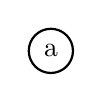
\begin{tikzpicture}[->, thick, node distance=2cm]
  \node[circle, draw] (a) {a};
\end{tikzpicture}

3. A = {a} and R = {(a,a)} \\
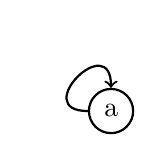
\begin{tikzpicture}[->, thick, node distance=2cm]
  \node[circle, draw] (a) {a};
  \draw (a.west) .. controls +(left:0.75cm) and +(up:0.75cm) .. (a.north);
\end{tikzpicture}

4. A = {a,b,c} and R = {(a,b),(a,c)} \\
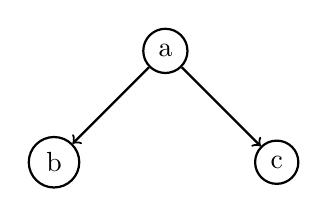
\begin{tikzpicture}[->, thick, node distance=2cm]
  \node[circle, draw] (a) {a};
  \node[circle, draw, below left of=a] (b) {b};
  \node[circle, draw, below right of=a] (c) {c};
  \draw (a) -- (b);
  \draw (a) -- (c);
\end{tikzpicture}

5. A = {a,b} and R = {(a,a),(a,b)} \\
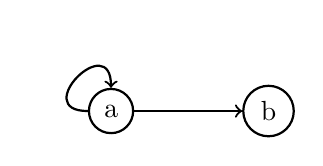
\begin{tikzpicture}[->, thick, node distance=2cm]
  \node[circle, draw] (a) {a};
  \node[circle, draw, right of=a] (b) {b};
  \draw (a) -- (b);
  \draw (a.west) .. controls +(left:0.75cm) and +(up:0.75cm) .. (a.north);
\end{tikzpicture}

6. A = {a,b,c} and R = {(a,b),(b,b)(a,c)} \\
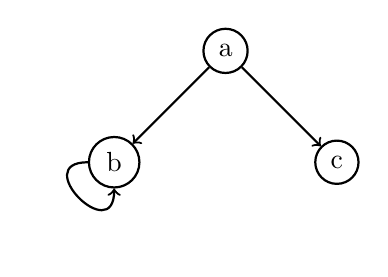
\begin{tikzpicture}[->, thick, node distance=2cm]
  \node[circle, draw] (a) {a};
  \node[circle, draw, below left of=a] (b) {b};
  \node[circle, draw, below right of=a] (c) {c};
  \draw (a) -- (b);
  \draw (b.west) .. controls +(left:0.75cm) and +(down:0.75cm) .. (b.south);
  \draw (a) -- (c);
\end{tikzpicture}

7. A = {a,b,c} and R = {(a,b),(b,b)(a,c),(c,c)} \\
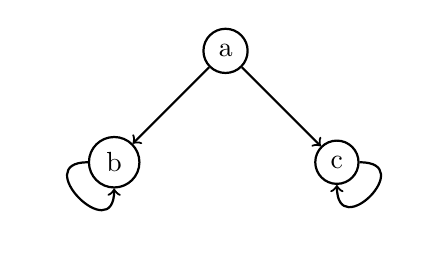
\begin{tikzpicture}[->, thick, node distance=2cm]
  \node[circle, draw] (a) {a};
  \node[circle, draw, below left of=a] (b) {b};
  \node[circle, draw, below right of=a] (c) {c};
  \draw (a) -- (b);
  \draw (a) -- (c);
  \draw (b.west) .. controls +(left:0.75cm) and +(down:0.75cm) .. (b.south);
  \draw (c.east) .. controls +(right:0.75cm) and +(down:0.75cm) .. (c.south);
\end{tikzpicture}


Try to find an example of an ARS for each of the possible 8 combinations of confluent, terminating, and has unique normal forms. Draw pictures of these examples.

T / T / T example: 

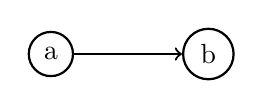
\begin{tikzpicture}[->, thick, node distance=2cm]
    \node[circle, draw] (a) {a};
    \node[circle, draw, right of=a] (b) {b};
    \draw (a) -- (b);
\end{tikzpicture}

T / T / F example: 

Cannot exist due the Theorem that If an ARS is confluent and terminating then all elements reduce to a unique normal form. Since this is both confluent and terminating, it must have a unique normal form.

T / F / T example: 

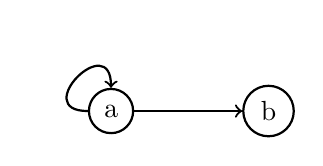
\begin{tikzpicture}[->, thick, node distance=2cm]
    \node[circle, draw] (a) {a};
    \node[circle, draw, right of=a] (b) {b};
    \draw (a) -- (b);
    \draw (a.west) .. controls +(left:0.75cm) and +(up:0.75cm) .. (a.north);
\end{tikzpicture}

T / F / F example: 

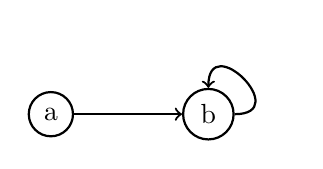
\begin{tikzpicture}[->, thick, node distance=2cm]
  \node[circle, draw] (a) {a};
  \node[circle, draw, right of=a] (b) {b};
  \draw (a) -- (b);
  \draw (b.east) .. controls +(right:0.75cm) and +(up:0.75cm) .. (b.north);
\end{tikzpicture}

F / T / T example: 

Confluent and having a unique normal form must be the same, one cannot be true while the other is false since an ARS has unique normal forms if and only if it is confluent and normalising.

F / T / F example: 

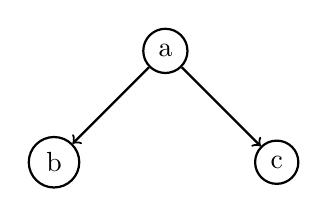
\begin{tikzpicture}[->, thick, node distance=2cm]
    \node[circle, draw] (a) {a};
    \node[circle, draw, below left of=a] (b) {b};
    \node[circle, draw, below right of=a] (c) {c};
    \draw (a) -- (b);
    \draw (a) -- (c);
\end{tikzpicture}

F / F / T example: 

Same as above, confluent and having a unique normal form must be the same, one cannot be true while the other is false since an ARS has unique normal forms if and only if it is confluent and normalising.

F / F / F example: 

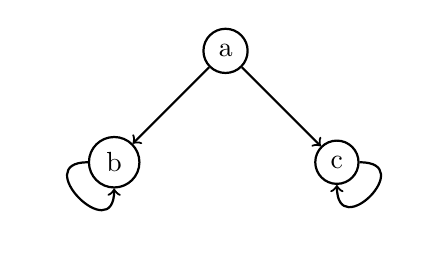
\begin{tikzpicture}[->, thick, node distance=2cm]
    \node[circle, draw] (a) {a};
    \node[circle, draw, below left of=a] (b) {b};
    \node[circle, draw, below right of=a] (c) {c};
    \draw (a) -- (b);
    \draw (a) -- (c);
    \draw (b.west) .. controls +(left:0.75cm) and +(down:0.75cm) .. (b.south);
    \draw (c.east) .. controls +(right:0.75cm) and +(down:0.75cm) .. (c.south);
\end{tikzpicture}

\subsubsection{Comments and Questions}

Since we can represent basic programs like bubble sort and XOR as an ARS, how does this help us understand the  logic and behavior of these programs better?

\subsection{Week 12}

\subsubsection{Notes}

This week explored the concept of invariants and their significance through different systems, such as mathematics and programming. Invariants are properties that do not change when we apply rules to the systems. Formally, this can be defined as a function $P: A \to B$ for an Abstract Reduction System (ARS) $(A, \to)$ such that if $a \to b$, then $P(a) = P(b)$ for all $a, b \in A$. This means that even when you apply the function $P$ to $a$ and $b$, they will still be equal to each other. 

An example of an invariant in an ARS is as follows: under the rule $ab \to ba$, invariants could include the total length of the string, the number of $a$'s or $b$'s, and the sum of $a$'s and $b$'s, since these are values that will never change no matter how the rule is applied. Strong invariants are symmetric and are the method of choice for studying equivalence classes, while weak invariants are appropriate if the direction of time is important.

Furthermore, if $P$ is an invariant property of the ARS $(A, \to)$ and $P(a) = \text{true}$ and $P(b) = \text{false}$, then $\neg (a \overset{*}{\to} b)$, $\neg (a \overset{*}{\leftarrow} b)$, and $a$ and $b$ are in different equivalence classes. Invariants can be used to demonstrate that certain transformations or operations are impossible by showing that two elements belong to different equivalence classes.


\subsubsection{Homework}
\begin{align*}
  \text{Rule: (fix (\textbackslash fact. \textbackslash n. if n=0 then 1 else n * fact (n-1))) $\rightarrow$ (fix (\textbackslash fact. \textbackslash n. if n=0))}
\end{align*}

\begin{align*}
  \text{let rec fact = \textbackslash n. if n=0 then 1 else n * fact (n-1) in fact 3} & \quad \mathbf{def\ of\ let\ rec} \\
  \text{let fact = (fix (\textbackslash fact. \textbackslash n. if n=0)) in fact 3} & \quad \mathbf{def\ of\ let} \\
  \text{(\textbackslash fact. fact 3) (fix (\textbackslash fact. \textbackslash n. if n=0))} & \quad \mathbf{beta\ rule:\ substitute\ fix\ F} \\
  \text{(fix (\textbackslash fact. \textbackslash n. if n=0)) 3} & \quad \mathbf{def\ of\ fix} \\
  \text{(\textbackslash fact. \textbackslash n. if n=0) (fix (\textbackslash fact. \textbackslash n. if n=0)) 3} & \quad \mathbf{beta\ rule:\ substitute\ fix\ F} \\
  \text{(\textbackslash n. if n=0 then 1 else n * (fix (\textbackslash fact. \textbackslash n1. if n1=0)) (n-1)) 3} & \quad \mathbf{beta\ rule:\ substitute\ 3} \\
  \text{if 3=0 then 1 else 3 * (fix (\textbackslash fact. \textbackslash n1. if n1=0)) (3-1)} & \quad \mathbf{def\ of\ if} \\
  \text{3 * (fix (\textbackslash fact. \textbackslash n1. if n1=0)) 2} & \quad \mathbf{def\ of\ fix} \\
  \text{3 * (\textbackslash fact. \textbackslash n1. if n1=0) (fix (\textbackslash fact. \textbackslash n1. if n1=0)) 2} & \quad \mathbf{beta\ rule:\ substitute\ fix\ F} \\
  \text{3 * (\textbackslash n1. if n1=0 then 1 else n1 * (fix (\textbackslash fact. \textbackslash n2. if n2=0)) (n1-1)) 2} & \quad \mathbf{beta\ rule:\ substitute\ 2} \\
  \text{3 * (if 2=0 then 1 else 2 * (fix (\textbackslash fact. \textbackslash n2. if n2=0)) (2-1))} & \quad \mathbf{def\ of\ if} \\
  \text{3 * (2 * (fix (\textbackslash fact. \textbackslash n2. if n2=0)) 1)} & \quad \mathbf{def\ of\ fix} \\
  \text{3 * (2 * (\textbackslash fact. \textbackslash n2. if n2=0) (fix (\textbackslash fact. \textbackslash n2. if n2=0)) 1)} & \quad \mathbf{beta\ rule:\ substitute\ fix\ F} \\
  \text{3 * (2 * (\textbackslash n2. if n2=0 then 1 else n2 * (fix (\textbackslash fact. \textbackslash n3. if n3=0)) (n2-1)) 1)} & \quad \mathbf{beta\ rule:\ substitute\ 1} \\
  \text{3 * (2 * (if 1=0 then 1 else 1 * (fix (\textbackslash fact. \textbackslash n3. if n3=0)) (1-1)))} & \quad \mathbf{def\ of\ if} \\
  \text{3 * (2 * (1 * (fix (\textbackslash fact. \textbackslash n3. if n3=0)) 0))} & \quad \mathbf{def\ of\ fix} \\
  \text{3 * (2 * (1 * (\textbackslash fact. \textbackslash n3. if n3=0) (fix (\textbackslash fact. \textbackslash n3. if n3=0)) 0))} & \quad \mathbf{beta\ rule:\ substitute\ fix\ F} \\
  \text{3 * (2 * (1 * (\textbackslash n3. if n3=0 then 1 else n3 * (fix (\textbackslash fact. \textbackslash n4. if n4=0)) (n3-1)) 0))} & \quad \mathbf{beta\ rule:\ substitute\ 0} \\
  \text{3 * (2 * (1 * (if 0=0 then 1 else 0 * (fix (\textbackslash fact. \textbackslash n4. if n4=0)) (0-1))))} & \quad \mathbf{def\ of\ if} \\
  \text{3 * (2 * (1 * 1))} & \quad \mathbf{def\ of\ *} \\
  \text{3 * (2 * 1)} & \quad \mathbf{def\ of\ *} \\
  \text{3 * 2} & \quad \mathbf{def\ of\ *} \\
  \text{6} &
\end{align*}


\subsubsection{Comments and Questions}

Are there any cases where a problem may not follow the invariant but still becomes solvable? Would that make the invariant invalid as a whole or would it just not be a good one?\ldots

\subsection{Week 13}
\subsubsection{Notes}

This week we loked a comparison of using insertion sort in different programming languages and also furthered our problem solving skills through analzying problems. 
While in different pgoramming languages the syntax is different, the overall idea behind how a function should work is the same. Through looking at it in multiple diffrerent languages,
we are able to gain a better understanding of how problem solving is the basis of coding. Two design criterias, simplicity and naturallity are important compromises that must be made
and are offened critiqued when it comes to building a language. The second part of class as analyzing two different problems and building a formula that would work to solve them.
The first one was "What the Tortoise Said to Achilles", in which the Tortoise challenges the basis of logical reasoning. In which, he refusies to accept a conclusion unless
and infinite number of justifications are provided, the Tortoise demonstarates an infinite regress problem in logic. The second one that we explored even deeper was the prisoner hat problem. 
The goal of this was to get at least (n being number of prisoners) n-1 / n of the prisoner's to say the correct hat color when they can only see x amount in front of them. Where x is all of the people who are shorter than them.
In class, we were able to create a reasonable answer of the first person, but were unable to give an easy formula for all the people following afterwards. 

\subsubsection{Homework}

Exercise 7: Consider the rewrite rules: \\
\begin{align*}
  ab &\rightarrow a \\
  bb &\rightarrow b \\
  aa &\rightarrow b
\end{align*}

Think of a and b as colours and an urn that has balls of colour a ("white") and b ("black"). Interpret the rewrite rules as rules about drawing balls from the urn. \\
- If one ball is white and one ball is black, replace them with a single white ball. \\
- If both are black, replace them with a single black ball. \\
- If both are white, replace them with a single black ball.

If you start with 198 black balls and 99 white balls, what is the colour of the last ball remaining? \\
- Since adding two white balls make a black ball, there would have to be an even number to have only black remaining. Since there are 99 white balls, an odd number of white balls, the last ball would stay and absorb all the black balls. 

The invariant for the problem is based on the parity of the white balls. If there are an even number of a's or white balls then, the final ball will be black but if it's odd then it will be white. \\
The unique normal form is that all properties will end up in either a, b, or empty set. If you start with an empty set then it will end up in empty set, but if you start with an even number of a's (including 0) then you will end up in a. However, if you start with an odd number of a's, then you will end up in b. 

If you start with n black balls and m white balls, the colour of the last ball will be based on this formula:
If \( m \mod 2 = 1 \), then white; else if \( m \mod 2 = 0 \), then black; else empty set.


\subsubsection{Comments and Questions}

If we started adding colors to the prisoners hat problem, are we able to determinate how many rules we have to add based on the number of colors?

\section{Lessons from the Group Assignments and Project}

\textbf{Programming Assignment 3:}

For Programming Assignment 3, I worked with Joseph Calise after both of us completed Exercises 0-9 
independently. Following this, I assisted with testing the program and structuring it in a way that 
ensured we both fully understood how the program was compiled and executed. This assignment helped us 
gain a foundational understanding of how a basic interpreter is created, particularly how it parses 
grammar to convert expressions into a format readable by the program. Additionally, I learned how the 
interpreter handles capture-avoiding substitution and how we adapted it to work for the minimum working 
examples and other test cases.

One technical challenge I faced was creating the minimum working example. Initially, I wasn’t sure 
where to start, so I sought help from Joseph, particularly for Exercise 5, which gave me the 
guidance needed to complete the rest of the assignment. During testing, we expanded beyond the 
provided test cases by creating additional examples for the program to evaluate. We analyzed whether 
the program would compile correctly or encounter errors by running it through various scenarios, 
including an artificial intelligence chatbot, to identify potential weaknesses.

Some theoretical concepts were particularly helpful in this assignment. For example, I learned 
how capture-avoiding substitution works by systematically renaming variables to prevent 
incorrect substitutions. Additionally, studying recursion stacks, such as in the Tower of Hanoi 
example, taught me how to build solutions incrementally. This approach informed our workflow: 
starting with the minimum working example and progressively building a functional program. 
If the program worked correctly for a smaller example, it was likely to handle larger, more 
complex cases as well.

Through this assignment, I developed a deeper understanding of how programs actually run. I 
realized that much of programming involves syntactic "sugar" layered over fundamental logic. 
Interpreters transform code into grammar that the system can process, rather than executing the 
code as written. This insight highlighted the similarities across programming languages, as many 
share the same core logic even when the syntax differs.

\textbf{Programming Assignment 4:}

For Programming Assignment 4, I worked with Joseph Calise, Greg Chinnici, and Quillan Gee throughout 
most of the project. This assignment built upon Programming Assignment 2, which served as our starting 
point. Instead of evenly dividing the work, we each began with our own tasks and collaborated to 
integrate our contributions into a single working solution. Using Discord, we were able to work 
independently and communicate effectively to complete the assignment.

The first milestone of this assignment involved creating a basic calculator that supported lambda 
functions and negation. Since Assignment 2 focused on similar functionality (excluding lambda functions), 
I was able to extend the grammar from the previous assignment. The main technical challenge here was 
ordering and naming the grammar rules to ensure that the program simplified expressions correctly 
without breaking or executing steps in the wrong order. Additionally, we had to create an evaluate 
function and a substitute function that worked correctly. We reused code from Assignment 3 as a 
foundation and extended it for this assignment, ensuring proper functionality. This milestone 
largely served as a review, combining concepts from the earlier assignments while introducing the 
new challenge of managing grammar precedence.

The second milestone required adding conditional statements, boolean expressions, and fixed-point 
combinators. While we were provided with an ambiguous grammar as a starting point, it was our task to 
order the grammar correctly so that the new features—conditional statements and boolean 
expressions—were processed before basic arithmetic operations. During this milestone, we again 
worked independently before coming together to finalize a solution. One significant challenge 
I faced was handling the fix function. Initially, it added everything into a new tuple instead of 
correctly modifying the existing one. Through class collaboration, our group discovered that applying 
fix using a lambda resolved the issue. From this milestone, we learned how to incorporate conditional 
statements, boolean expressions, and fixed-point combinators into the calculator, as well as how the 
evaluate function processed inputs and returned tuples. The fix function in particular helped us better
understand how the interpreter handled recursive evaluation.

The third milestone involved adding sequencing and operations for constructing and destructing lists. 
Like the previous milestone, we worked independently during a break and reconvened in class to address 
challenges. A key technical issue was ensuring the program treated lists as single entities rather 
than reading them as separate elements (e.g., a number and a list). Joseph addressed this challenge 
by creating a preprocessor that used regular expressions to identify lists and wrap them in parentheses 
as tuples. Using debugging techniques, such as setting breakpoints and running the code line by line,
I identified issues related to the substitution of head and tail due to missing elif statements. This 
milestone further enhanced my understanding of the evaluate and substitute functions and how programs 
create and interact with different data types. Whether it was developing the preprocessor or modifying 
the grammar to handle lists, this milestone demonstrated how interpreters process inputs and produce 
consistent outputs, even when the internal mechanisms vary.

One unresolved challenge was debugging the insertion sort implementation. While we couldn't identify 
the exact issue, running the code line by line helped us trace the problem to the evaluate function.
Despite this, we gained valuable insights into how the program processed different data types and 
how outputs were generated. Understanding these processes was the most significant takeaway from this 
milestone.

\textbf{Conclusion:}

Through Programming Assignments 3 and 4, I gained a solid understanding of interpreters, including 
key concepts like capture-avoiding substitution, recursion, and grammar precedence. Collaborating 
with my peers taught me the importance of combining individual efforts into a cohesive solution 
while tackling challenges like fix evaluation and list processing. These projects strengthened 
my understanding of programming language mechanics and how theory informs practical implementation, 
lessons I will apply to future work.

\section{Conclusion}\label{conclusion}

While this course was challenging, particularly in the theoretical portions, I was able to understand 
most of the topics and how they connect to the wider world of software engineering. Through this 
course, we explored how proofs are created to prove theorems about math and how those concepts apply 
to the programs we create. Most importantly, we learned to use recursion to simplify programs into 
smaller versions of themselves. Other topics we covered included parsing, higher-order functions, and 
Turing completeness. These concepts are essential to software engineering because parsing enables us 
to read calls for functions through inputs and return outputs, higher-order functions allow us to 
insert functions to output another function, and Turing completeness helps us prove that programs or 
computations are theoretically calculable. While some topics were easier to understand than others, 
everything came together during programming assignment 4, where I could see how all the concepts 
coincided into one cohesive course. The course explained well how programming languages read the 
programs we write and how syntactical sugar is created. At the core, most programs run similarly 
but interpret syntax differently based on their documentation. This process involves parsing the 
program into functions and inserts, evaluating them, and sometimes substituting different values, 
as we did in programming assignments 2 through 4. These steps reinforced how theoretical ideas 
translate into practical tools for building software. Among all the topics, I found invariants and 
puzzle-solving to be the most interesting since I love brain teasers. Invariants introduced a new way 
to approach puzzles—not just by searching for answers but by understanding why answers might not exist or 
finding examples where solutions aren't possible. For example, invariants let me view problems from a different 
angle, identifying patterns and constraints that I might have missed otherwise. However, learning about invariants 
earlier in the course wouldn’t have worked because we needed foundational tools to define and solve puzzles effectively. 
One unique aspect of the course was the restriction on using laptops for note-taking during lectures. This 
required us to focus on remembering concepts discussed in class rather than relying solely on written notes. 
While this was useful in some ways, I would suggest either allowing laptops strictly for note-taking or updating 
the online notes to reflect any additional ideas explored during lectures. This would make it easier to reference 
concepts later and ensure no important details are missed. Overall, this course gave me a better understanding of 
how programming languages function and how theoretical concepts apply to practical software engineering. While it 
was challenging at times, the integration of theory and application made it a valuable experience that ties 
directly into the wider world of software engineering.

\begin{thebibliography}{99}
\bibitem[label]{citekey} Andrew Moshier, \href{https://canvas.chapman.edu/courses/66029/files/6581500?module_item_id=2280521}{Contemporary Discrete Mathematics}, M\&H Publishing, 2024
\end{thebibliography}

\end{document}
